\documentclass[12pt]{article}
\usepackage{mathematics}

\begin{document}

\subsection*{1A}
\begin{mdframed}
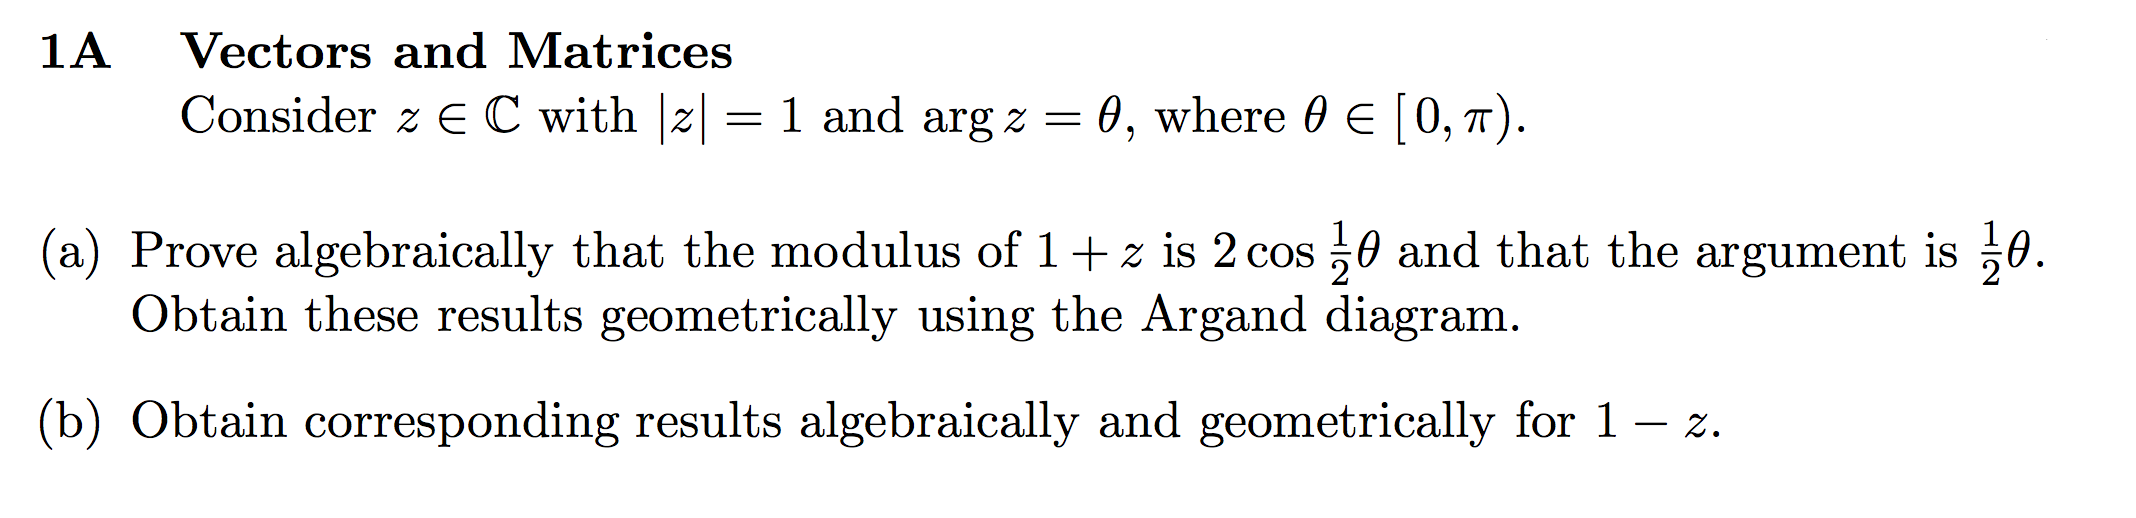
\includegraphics[width=400pt]{img/misc--cambridge-1a-2017-1-1A.png}
\end{mdframed}
\begin{proof}(Algebraic)\\
Note that
$\cos\theta = \cos^2\frac{1}{2}\theta - \sin^2\frac{1}{2}\theta = 2\cos^2\frac{1}{2}\theta - 1$.

We have $z = \cos\theta + i\sin\theta$ and therefore
\begin{align*}
  |1 + z|  &= \sqrt{(1 + \cos\theta)^2 + \sin^2\theta}
             = \sqrt{2(1 + \cos\theta)}
             = \sqrt{2\Big(1 + 2\cos^2\frac{1}{2}\theta - 1\Big)}
             = 2\cos\frac{1}{2}\theta\\
  |1 - z| &= \sqrt{(1 - \cos\theta)^2 + \sin^2\theta}
            = \sqrt{2(1 - \cos\theta)}
            = \sqrt{2(1 - (2\cos^2\frac{1}{2}\theta - 1))}
            = 2\sin\frac{1}{2}\theta.
\end{align*}
\end{proof}

\begin{proof}(Geometric)\\
  \begin{mdframed}
    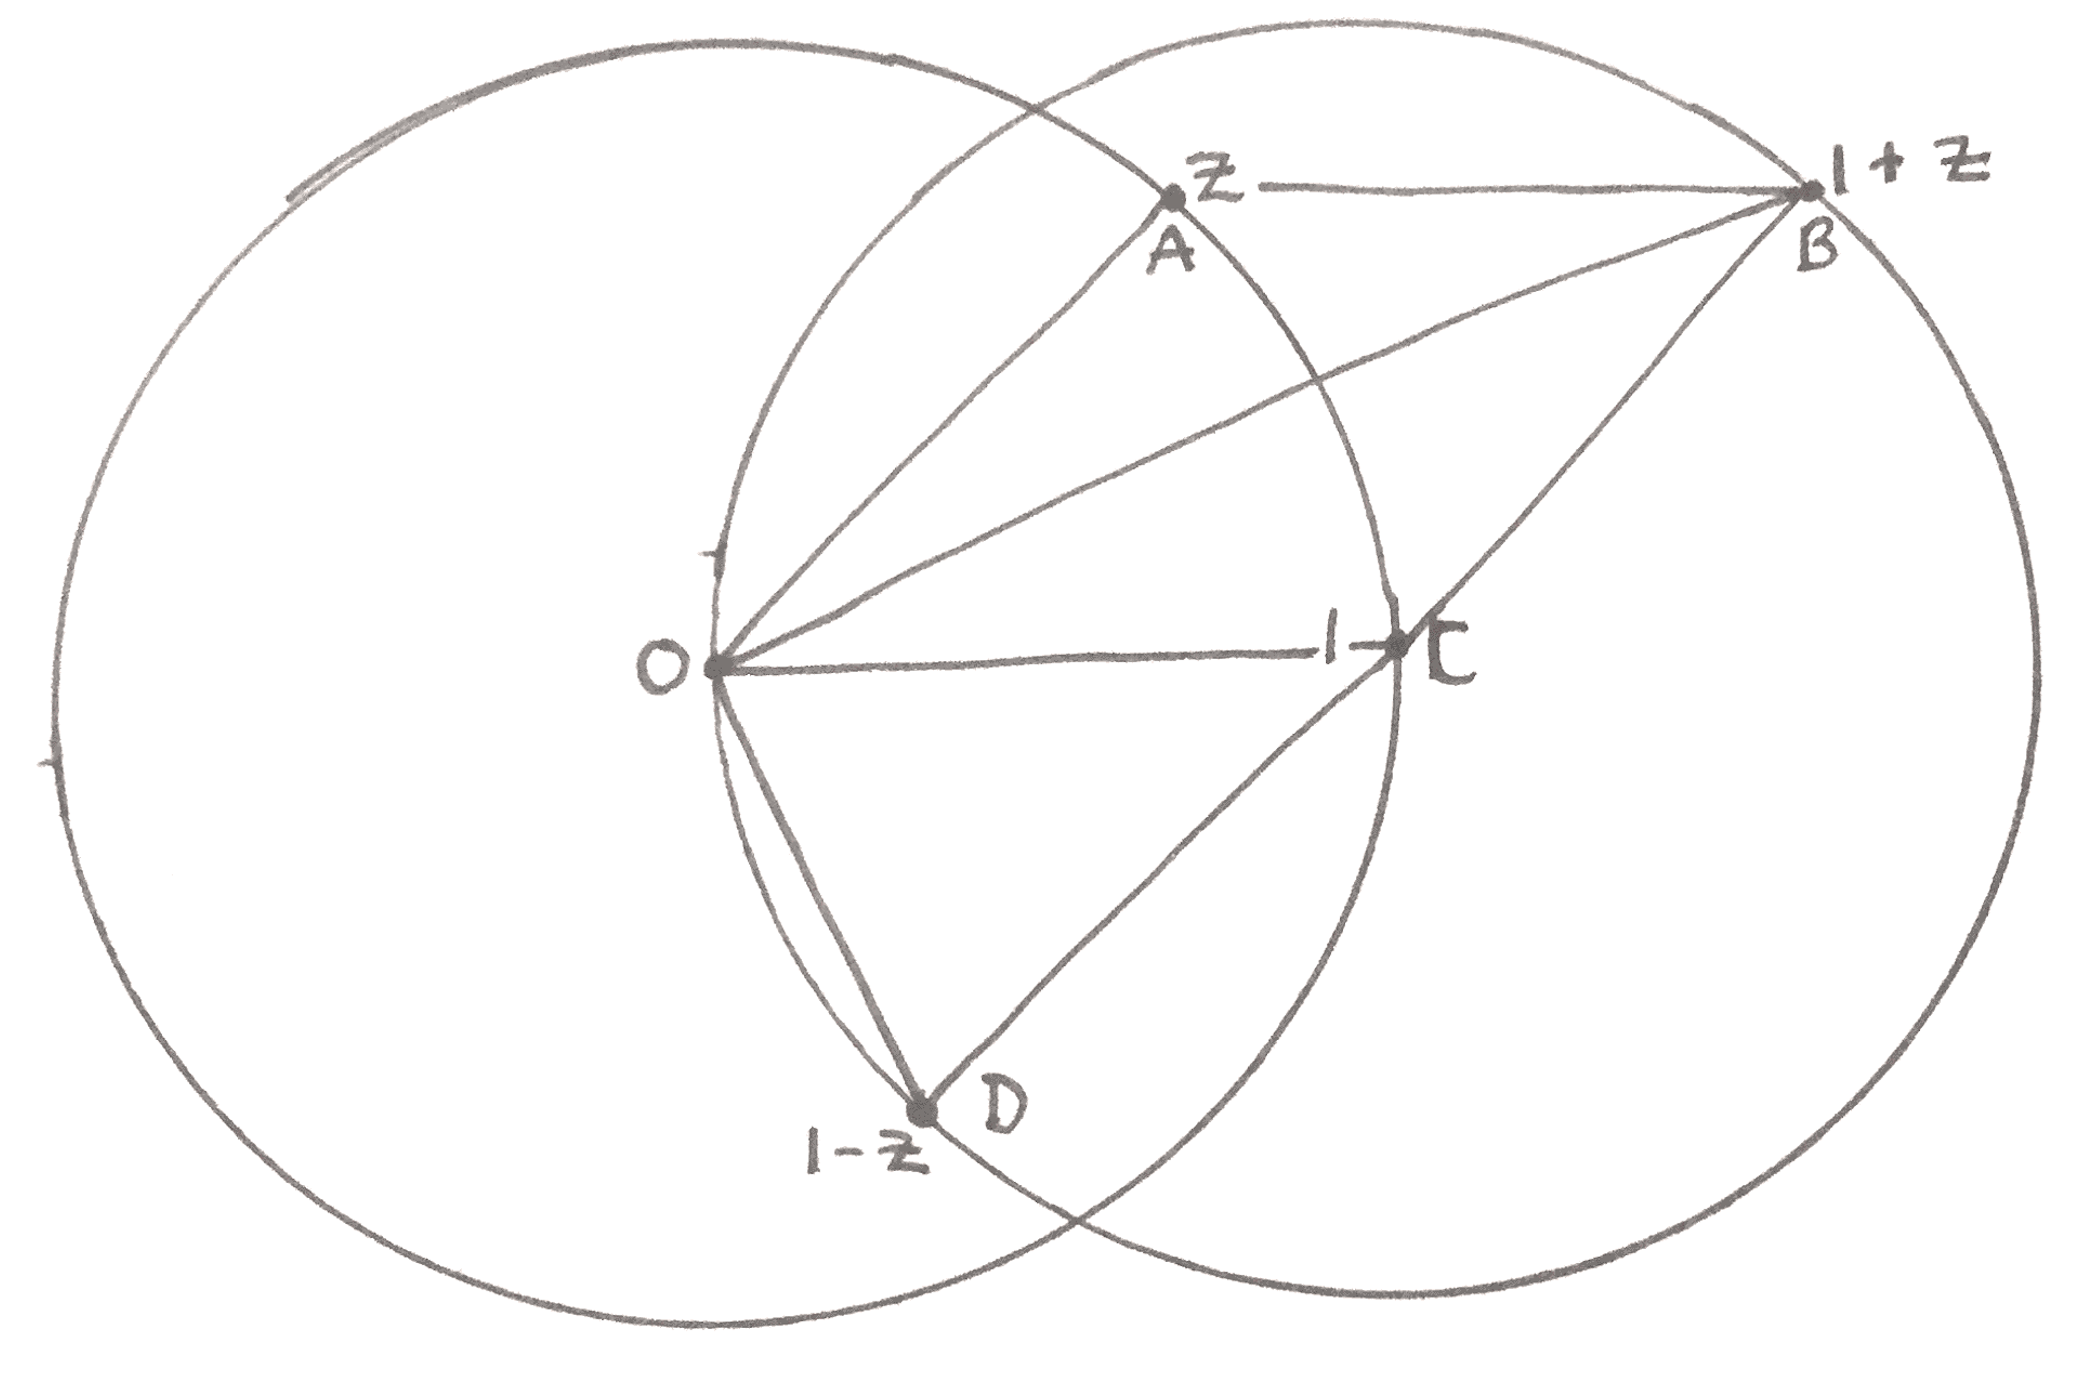
\includegraphics[width=300pt]{img/misc--cambridge-1a-2017-1-1A-diagram.png}
  \end{mdframed}
  $OABC$ is a rhombus, with sides of length 1 and $\angle AOC=\theta$. The diagonal $OB$ bisects
  $\angle AOC$, therefore $\angle OBC = \theta/2$. $\angle BOD$ is a right angle since it is formed
  from a triangle inscribed in a circle. Hypotenuse $BD$ has length 2, since $C$ is the centre of a
  second unit circle with radii $CB$ and $CD$. Therefore the length of $OB$ is
  $2\cos\frac{1}{2}\theta$ and the length of $OD$ is $2\sin\frac{1}{2}\theta$.
\end{proof}


\newpage
\subsection*{2C}
\begin{mdframed}
  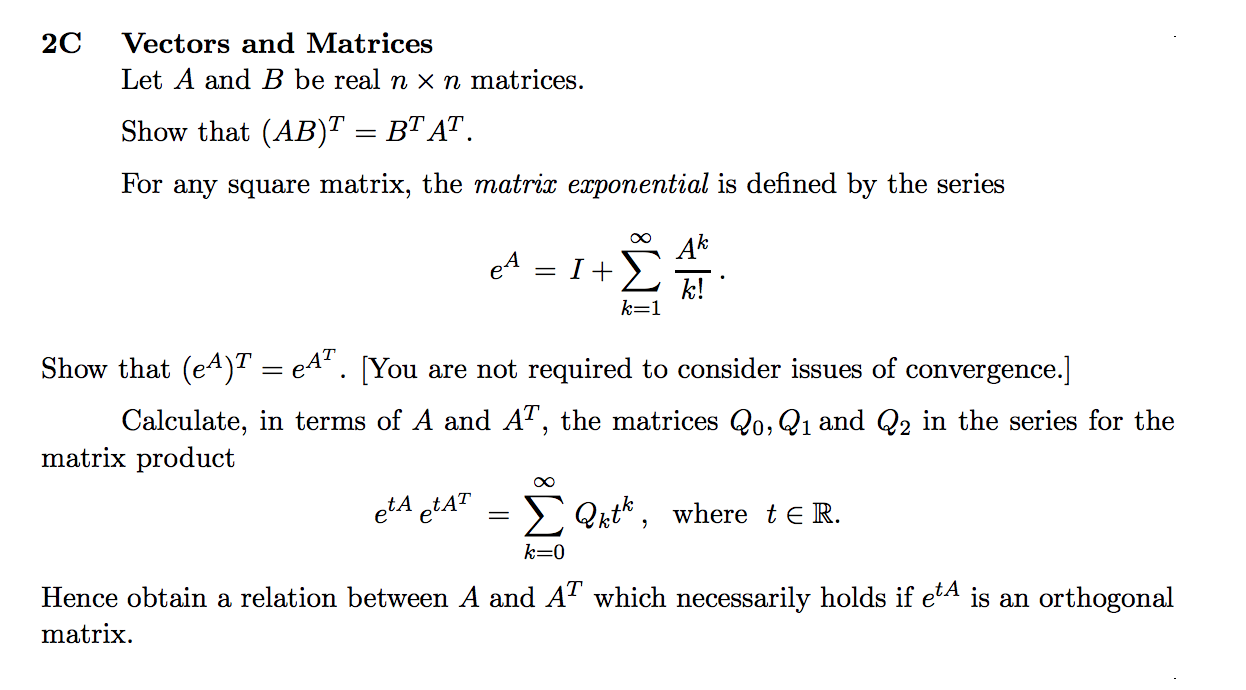
\includegraphics[width=400pt]{img/misc--cambridge-1a-2017-1-2c.png}
\end{mdframed}

\begin{claim*}
  $(AB)^T = B^TA^T$
\end{claim*}

\begin{proof}
  Let $i, j \in \{1, \ldots, n\}$. Then
  \begin{align*}
    \((AB)^T\)_{ij} = (AB)_{ji}
                   = \sum_{l=1}^n A_{jl}B_{li}
                   = \sum_{l=1}^n (A^T)_{lj}(B^T)_{il}
                   = (B^TA^T)_{ij}
  \end{align*}
\end{proof}

\begin{lemma*}
  $(A^k)^T = (A^T)^k$.
\end{lemma*}

\begin{proof}
  Note that $(A^m)^T(A^T)^n = (AA^{m-1})^T(A^T)^n = (A^{m-1})^T(A^T)^{n+1}$. By iterating this
  formal manipulation $k$ times, we have $(A^k)^T = (A^k)^T(A^T)^0 = (A^0)^T(A^T)^k = (A^T)^k$.
\end{proof}

\newpage
\begin{claim*}
  $(e^A)^T = e^{(A^T)}$
\end{claim*}

\begin{proof}
  Note that $(e^A)_{ij} := \sum_{k=0}^\infty \frac{(A^k)_{ij}}{k!}$, where $A^0 := I$ and
  $0! := 1$.  Therefore
  \begin{align*}
    \((e^A)^T\)_{ij} = \sum_{k=0}^\infty \frac{((A^k)^T)_{ij}}{k!}
                    = \sum_{k=0}^\infty \frac{((A^T)^k)_{ij}}{k!}
                    = \(e^{(A^T)}\)_{ij} .
  \end{align*}
\end{proof}

\begin{problem*}
  For $t \in \R$ we define matrices $Q_k$ such that $e^{tA}e^{tA^T} = \sum_{k=0}^\infty
  Q_kt^k$. Calculate $Q_0, Q_1, Q_2$.
\end{problem*}

\begin{proof}[Solution]~\\
  Note that
  \begin{align*}
    e^{tA}e^{tA^T}
    &=
      \(\sum_{k=0}^\infty\frac{(tA)^k}{k!}\)
      \(\sum_{k=0}^\infty \frac{(tA^T)^k}{k!}\)\\
    &=
      \(\sum_{k=0}^\infty\frac{t^k}{k!}A^k\)
      \(\sum_{k=0}^\infty \frac{t^k}{k!}(A^k)^T\).
  \end{align*}
  Therefore, by considering the coefficients of $t^0, t^1$ and $t^2$ in the expansion,
  \begin{align*}
    Q_0 &= I\\
    Q_1 &= A + A^T\\
    Q_2 &= AA^T + \frac{1}{2}(A^2 + (A^2)^T).
  \end{align*}

  If $e^{tA}$ is orthogonal, then
  $e^{tA}e^{tA^T} = e^{tA}e^{((tA)^T)} = e^{tA}(e^{tA})^T = e^{tA}(e^{tA})^\1 = I = \sum_{k=0}^\infty Q_kt^k$.

  Therefore $\sum_{k=1}^\infty Q_kt^k = 0$ for all $t$.

  Therefore $Q_k = 0$ for $k \in \{1, 2, \ldots\}$ \red{TODO: proof}.

  In particular, $Q_1 = 0$, therefore $A^T = -A$.

  As a check, we have $Q_2 = -A^2 + \frac{1}{2}(A^2 + (-A)^2) = 0$, as required.
\end{proof}

\newpage
\subsection*{3F}
\begin{mdframed}
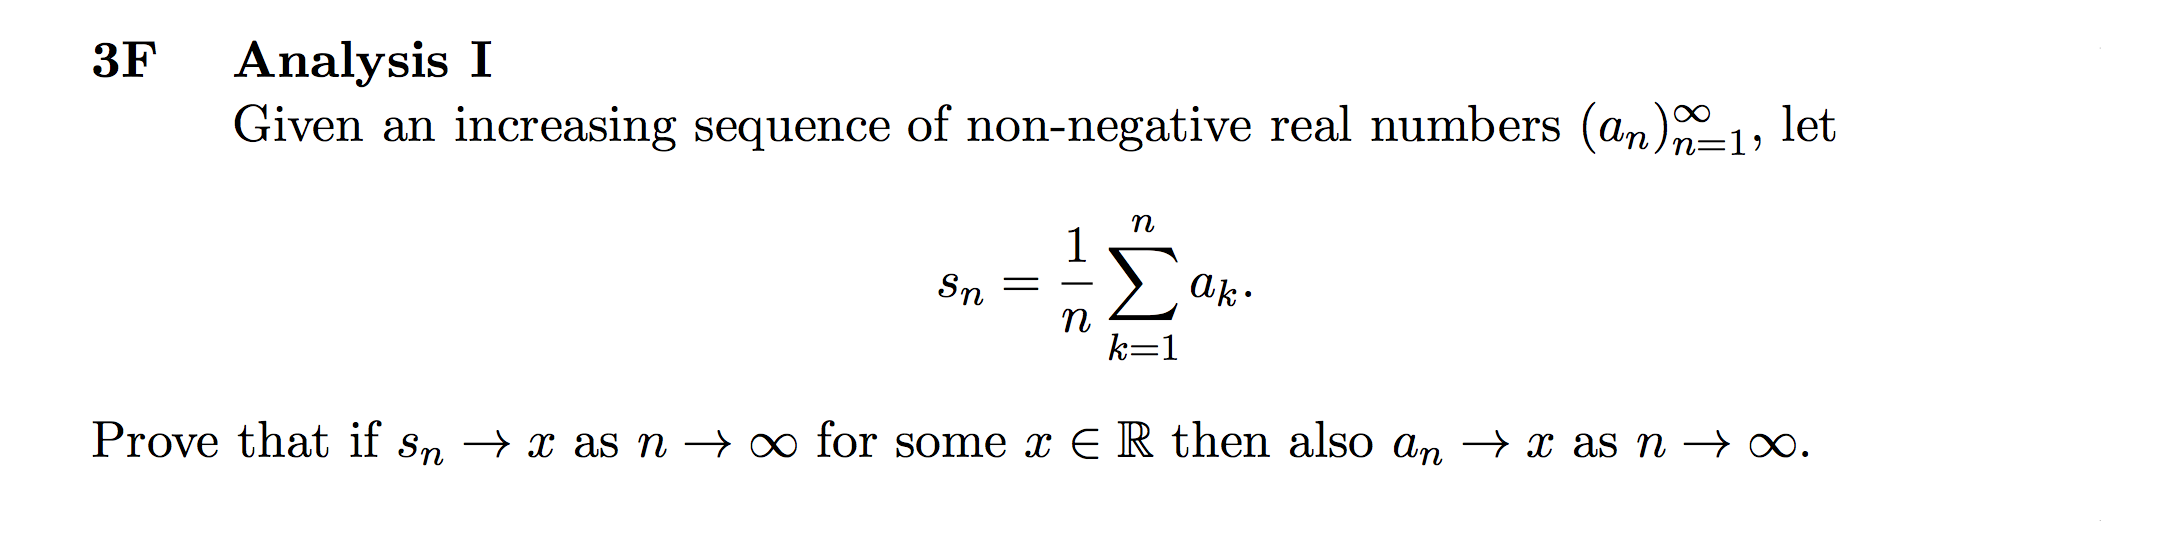
\includegraphics[width=400pt]{img/misc--cambridge-1a-2017-1-3f.png}
\end{mdframed}

\begin{proof}
  Assume that $s_n \to x$ as $n \to \infty$. We will show that $s_n \leq a_n \leq x$, for all $n$,
  therefore $a_n \to x$ as $n \to \infty$, as required.

  First note that $s_{n+1} = \frac{n}{n+1}s_n + \frac{1}{n+1}a_{n+1}$.
  % Note that $s_{n+1} = \frac{1}{n+1}\(\sum_{k=1}^na_k + a_{n+1}\) = \frac{n}{n+1}s_n + \frac{1}{n+1}a_{n+1}$.

  It's intuitively obvious that $s_n \leq a_n$ for all $n$. To prove this, note that it's true for
  $n = 1$; assume for induction that it's true for $n = k$. Then we have
  $s_{k+1} = \frac{k}{k+1}s_k + \frac{1}{k+1}a_{k+1} \leq \frac{k}{k+1}a_k + \frac{1}{k+1}a_{k+1}
  \leq a_{k+1}$, as required.

  Finally we show that $a_n \leq x$ for all $n$. Seeking a contradiction, assume that there exists
  $M$ such that $a_M > x$. Let $\epsilon = a_M - x > 0$, so that $a_n > x + \epsilon$ for $n > M$
  (see diagram). Then for $n > M$ we have
  \begin{align*}
    s_n &= \frac{1}{n}\sum_{k=1}^M a_k + \frac{1}{n}\sum_{k=M+1}^n a_k\\
        &> \frac{1}{n}\sum_{k=1}^M a_k + \frac{n - M}{n}(x + \epsilon).
  \end{align*}
  Therefore $\lim_{n\to\infty}s_n > x + \epsilon$ which is a contradiction, proving that
  $a_n \leq x$ for all $n$.
\begin{mdframed}
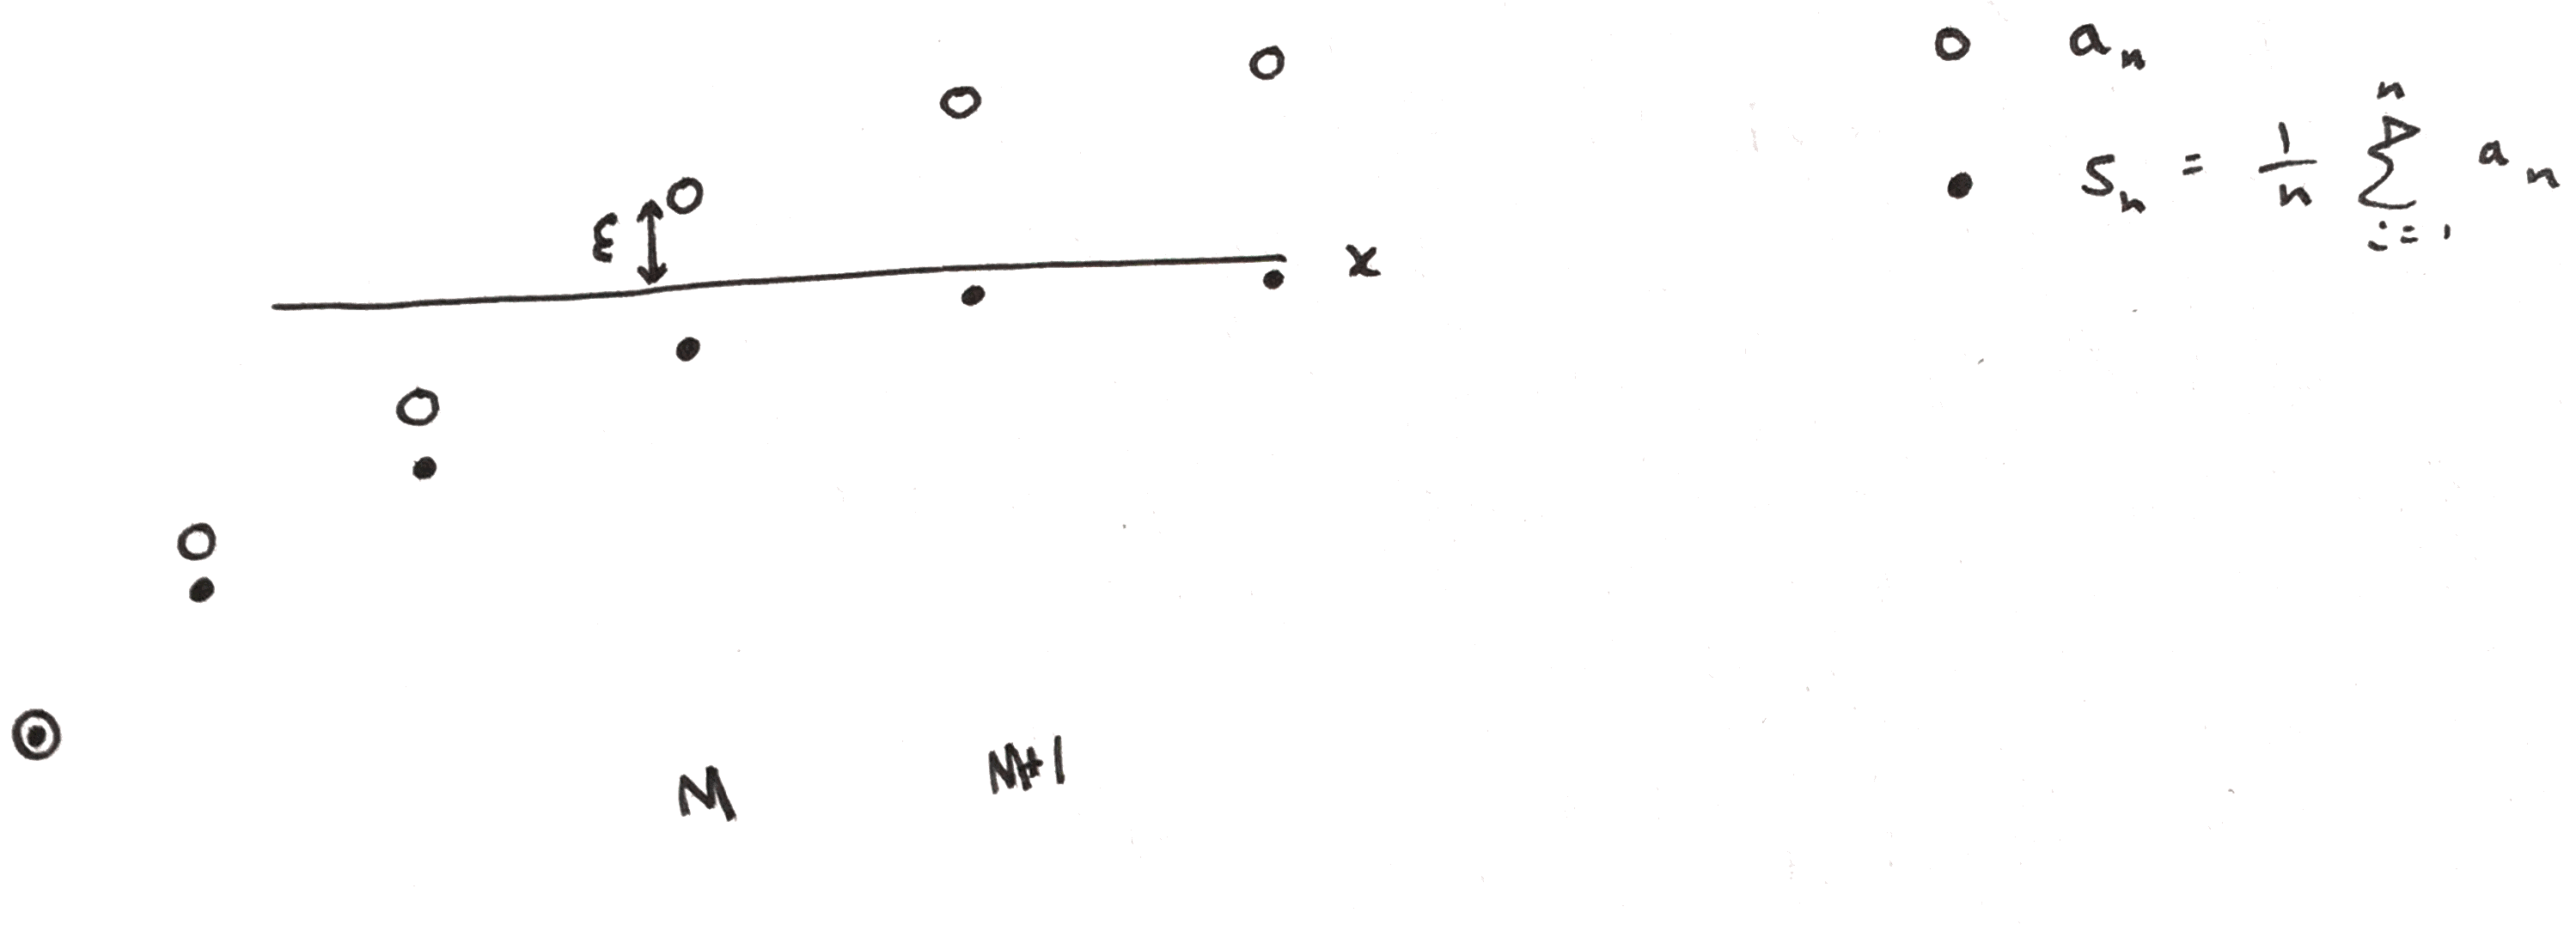
\includegraphics[width=400pt]{img/misc--cambridge-1a-2017-1-3f-diagram.png}
\end{mdframed}
\end{proof}



\begin{mdframed}
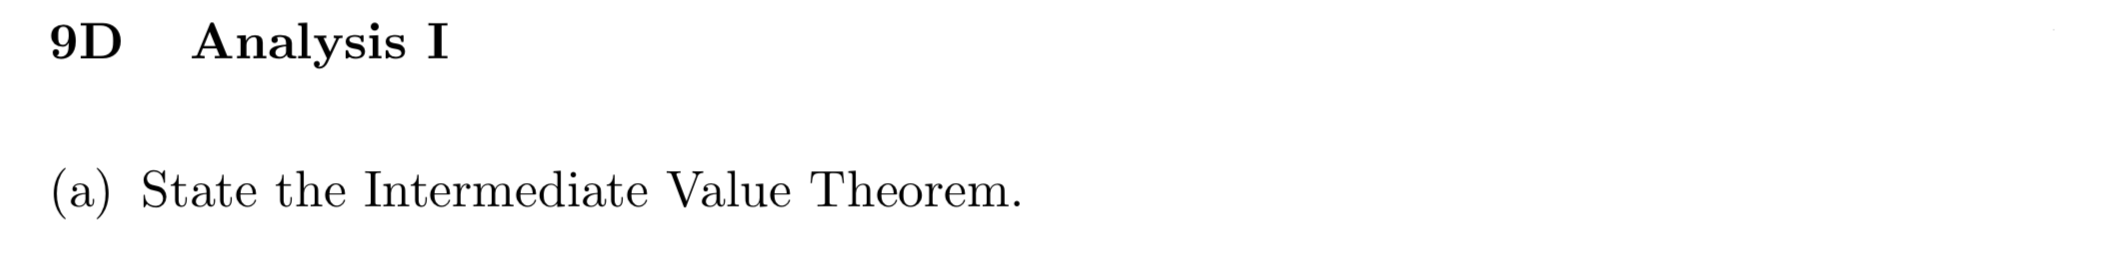
\includegraphics[width=400pt]{img/misc--cambridge-1a-2017-1-9D-1.png}
\end{mdframed}


\begin{theorem*}[Intermediate Value Theorem]~\\
  Let $a, b \in \R$, and $f:[a, b] \to \R$ be continuous. Let $y$ lie strictly between $f(a)$ and
  $f(b)$. Then there exists $x \in (a, b)$ such that $f(x) = y$.
\end{theorem*}

\begin{proof}
  % Use continuity of $f$ and completeness of $\R$ (every non-empty subset with upper bound has
  % supremum).

  Define $S = \{x \in [a, b] ~|~ f(x) < y\}$.

  Note that $a \in S$ so $S \neq \emptyset$, and $S$ bounded above by $b$ so $\sup S$ exists, by
  completeness of the reals.

  Put $t = \sup S$.

  Claim: $f(t) = u$.

  % Since $f$ is continuous, we have $\lim_{x \to t}f(x) = f(t)$.

  % So claim: $\lim_{x \to t}f(x) = u$.

  % Proof:

  Claim: for all $\epsilon > 0$, we have $u - \epsilon < f(t) < u + \epsilon$.

  Proof:

  Let $\epsilon > 0$.

  Since $f$ is continuous at $t$, we have that there exists $\delta$ such that
  \begin{align} \label{1}
    |x - t| < \delta \implies |f(x) - f(t)| < \epsilon.
  \end{align}

  I.e.
  \begin{align*}
    t - \delta < x < t + \delta \implies f(t) - \epsilon < f(x) < f(t) + \epsilon.
  \end{align*}

  Note that $t - \delta$ is not an upper bound for $S$.

  Therefore there exists $a^* > t - \delta$ such that $a^* \in S$.

  As $a^* \in S$, we have $a^* \leq t$.

  Therefore $a^* \in (t - \delta, t] \subseteq (t - \delta, t + \delta)$.

  By \eqref{1} we have $f(t) - \epsilon < f(a^*) < f(t) + \epsilon$.

  Since $a^* \in S$ we have $f(a^*) < u$.

  Therefore $f(t) - \epsilon < f(a^*) < u$.

  Therefore $f(t) < u + \epsilon$.

  Let $a^{**} \in (t, t + \delta)$.

  Since $a^{**} > t$, we have $a^{**} \notin S$.

  Therefore $f(a^{**}) \geq u$, i.e. $u < f(a^{**})$.

  Also by \eqref{1} we have $f(t) - \epsilon < f(a^{**}) < f(t) + \epsilon$, since
  $a^{**} \in (t - \delta, t + \delta)$.

  Therefore $u < f(t) + \epsilon$, i.e. $f(t) > u - \epsilon$.

  So we have $f(t) < u + \epsilon$ and $f(t) > u - \epsilon$, so

  $u - \epsilon < f(t) < u + \epsilon$ for all $\epsilon > 0$, therefore $f(t) = u$.
\end{proof}


% \begin{proof}
%   Use continuity of $f$ and completeness of $\R$ (every non-empty subset with upper bound has
%   supremum).

%   Define $S = \{x \in [a, b] ~|~ f(x) < a\}$.

%   Note $a \in S$, $S$ bounded above by $b$ so $\sup S$ exists.

%   Put $t = \sup S$.

%   Claim: $f(t) = u$.

%   Claim: $\lim_{x\to t} f(x) = u$.

%   Let $\epsilon > 0$.

%   Since $f$ is continuous at $t$, $\lim_{x \to t} f(x) = f(t)$.

%   Therefore there exists $\delta > 0$ such that
%   $|x - t| < \delta \implies |f(x) - f(t)| < \epsilon$.

%   (Including $x = t$.)

%   Recall that $t$ is an upper bound for $S$.

%   Hence $x > t \implies f(x) \geq u$.

%   Claim 1: $x < t \implies f(x) \leq u$.

%   Proof 1: $x < t \implies x \in S \implies f(x) < u$.

%   ~\\

%   Claim 2: $x > t \implies f(x) \geq u$.

%   Proof 2:



% \end{proof}

\begin{mdframed}
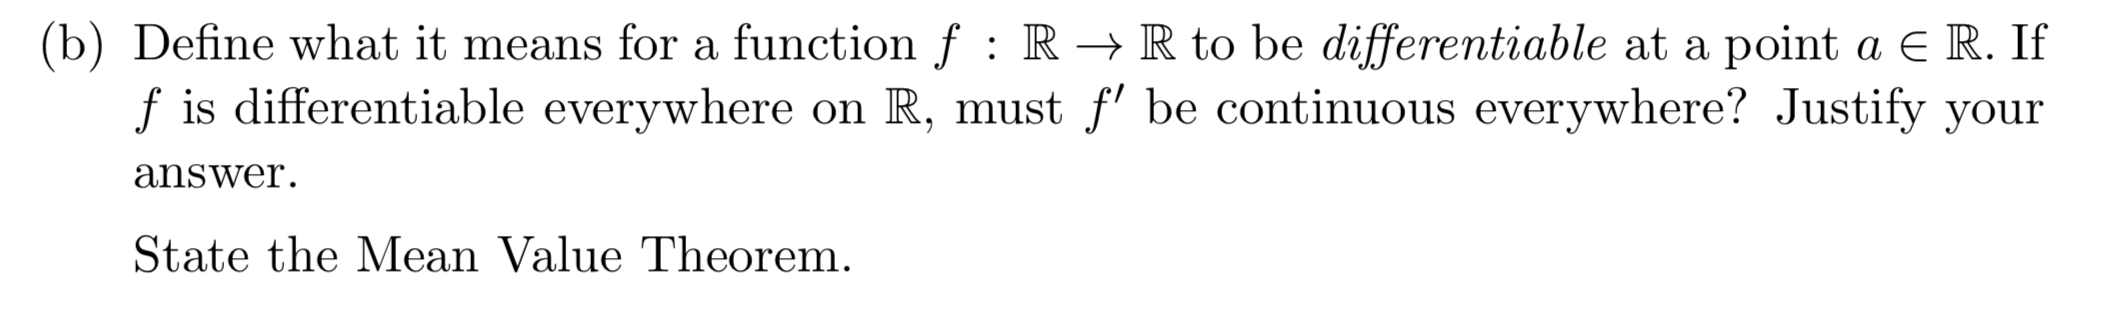
\includegraphics[width=400pt]{img/misc--cambridge-1a-2017-1-9D-2.png}
\end{mdframed}

\begin{definition*}
  Let $f: \R \to \R$ and $a \in \R$. If the limits
  \begin{align*}
    \lim_{x \to a^+} \frac{f(x) - f(a)}{x - a}\\
    \lim_{x \to a^-} \frac{f(x) - f(a)}{x - a}
  \end{align*}
  both exist and are equal then $f$ is differentiable at $a$.
\end{definition*}

We seek a counterexample: a function that is differentiable everywhere on $\R$ but $f'$ is not
continuous everywhere.



\end{document}
